\documentclass[tikz,border=4pt]{standalone}
% Shared visual grammar: role fills, dark connectors, and 7-point typography.
% Build each standalone figure from this directory. No external images required.
\pdfinfoomitdate=1
\pdftrailerid{}
\usepackage[T1]{fontenc}
\usepackage{helvet}
\renewcommand{\familydefault}{\sfdefault}
\usepackage{amsmath,amssymb}
\hyphenpenalty=10000
\exhyphenpenalty=10000
\usetikzlibrary{arrows.meta,calc,fit,positioning,decorations.pathreplacing,backgrounds}
\definecolor{ink}{HTML}{172B3A}
\definecolor{muted}{HTML}{586D85}
\definecolor{datafill}{HTML}{F1F5F9}
\definecolor{dataline}{HTML}{62748E}
\definecolor{modelfill}{HTML}{E5E9FF}
\definecolor{modelline}{HTML}{7887C7}
\definecolor{llmfill}{HTML}{FFE4E8}
\definecolor{llmline}{HTML}{E68494}
\definecolor{truthfill}{HTML}{D0FAE5}
\definecolor{truthline}{HTML}{35A782}
\newcommand{\seven}{\fontsize{7}{8.5}\selectfont}
\tikzset{
 every node/.append style={font=\seven,text=ink,align=center},
 box/.style={draw=dataline,fill=white,rounded corners=3pt,line width=.65pt,inner sep=5pt,minimum height=8mm},
 data/.style={box,fill=datafill},
 model/.style={box,draw=modelline,fill=modelfill},
 llm/.style={box,draw=llmline,fill=llmfill},
 truth/.style={box,draw=truthline,fill=truthfill},
 title/.style={font=\seven\bfseries,inner sep=1pt},
 word/.style={text=muted,inner sep=1pt,align=center},
 label/.style={fill=white,inner xsep=2pt,inner ysep=1pt,text=muted},
 flow/.style={-{Stealth[length=2.4mm,width=1.9mm]},draw=ink,line width=1.2pt,shorten >=1.5pt},
 branch/.style={-{Stealth[length=2mm,width=1.6mm]},draw=ink,line width=.9pt,shorten >=1pt},
 route/.style={draw=ink,line width=1.2pt},
 update/.style={-{Stealth[length=2.2mm,width=1.7mm]},draw=modelline,line width=1pt,dash pattern=on 3pt off 2pt,shorten >=1.5pt},
 boundary/.style={draw=dataline,dash pattern=on 3pt off 2pt,rounded corners=3pt,line width=.6pt},
 chip/.style={minimum height=4mm,inner xsep=3pt,inner ysep=1.5pt,rounded corners=2pt},
}
% Optional role key. Anchor at the center of an uncluttered final row.
\newcommand{\rolekey}[2]{
 \node[word,anchor=east] at (#1-6.6,#2) {\textit{Key}};
 \node[data,chip] at (#1-5.2,#2) {records / data};
 \node[model,chip] at (#1-1.9,#2) {learned model / policy};
 \node[llm,chip] at (#1+1.65,#2) {LLM signal};
 \node[truth,chip] at (#1+4.95,#2) {labels / evaluation};
}

\begin{document}
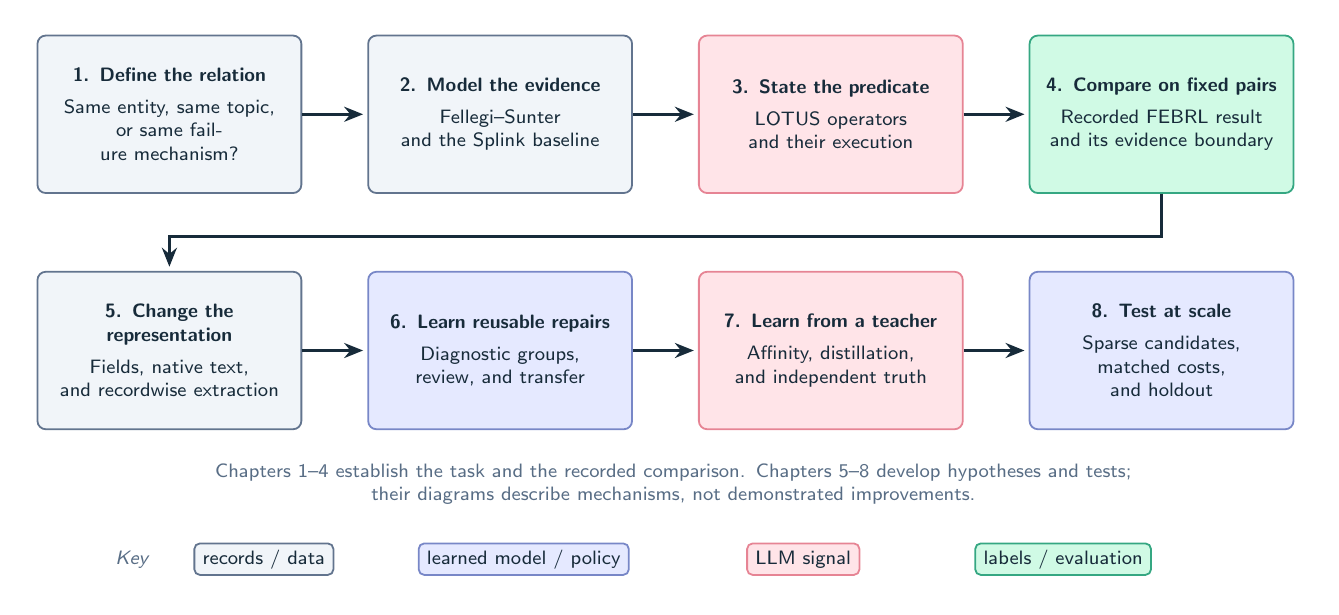
\begin{tikzpicture}

\useasboundingbox (-.2,.3) rectangle (16.1,-6.8);
\node[data,text width=30mm,minimum height=20mm] (c1) at (1.6,-.8) {\textbf{1. Define the relation}\\[3pt]Same entity, same topic,\\or same failure mechanism?};
\node[data,text width=30mm,minimum height=20mm] (c2) at (5.8,-.8) {\textbf{2. Model the evidence}\\[3pt]Fellegi--Sunter\\and the Splink baseline};
\node[llm,text width=30mm,minimum height=20mm] (c3) at (10,-.8) {\textbf{3. State the predicate}\\[3pt]LOTUS operators\\and their execution};
\node[truth,text width=30mm,minimum height=20mm] (c4) at (14.2,-.8) {\textbf{4. Compare on fixed pairs}\\[3pt]Recorded FEBRL result\\and its evidence boundary};
\draw[flow] (c1) -- (c2); \draw[flow] (c2) -- (c3); \draw[flow] (c3) -- (c4);
\node[data,text width=30mm,minimum height=20mm] (c5) at (1.6,-3.8) {\textbf{5. Change the representation}\\[3pt]Fields, native text,\\and recordwise extraction};
\node[model,text width=30mm,minimum height=20mm] (c6) at (5.8,-3.8) {\textbf{6. Learn reusable repairs}\\[3pt]Diagnostic groups,\\review, and transfer};
\node[llm,text width=30mm,minimum height=20mm] (c7) at (10,-3.8) {\textbf{7. Learn from a teacher}\\[3pt]Affinity, distillation,\\and independent truth};
\node[model,text width=30mm,minimum height=20mm] (c8) at (14.2,-3.8) {\textbf{8. Test at scale}\\[3pt]Sparse candidates,\\matched costs, and holdout};
\draw[flow] (c4.south) -- (14.2,-2.35) -- (1.6,-2.35) -- (c5.north);
\draw[flow] (c5) -- (c6); \draw[flow] (c6) -- (c7); \draw[flow] (c7) -- (c8);
\node[word,text width=135mm] at (8,-5.5) {Chapters 1--4 establish the task and the recorded comparison. Chapters 5--8 develop hypotheses and tests;\\their diagrams describe mechanisms, not demonstrated improvements.};
\rolekey{8}{-6.45}

\end{tikzpicture}
\end{document}
